\documentclass{article}

\usepackage{amsfonts}
\usepackage{amsthm}
\usepackage{mathrsfs}
\usepackage{amsmath}
\usepackage{graphicx}
\usepackage{hyperref}
\usepackage{stackengine}
\usepackage[mathscr]{eucal}
\usepackage{listings}
\usepackage{algorithm}
\usepackage{algpseudocode}
\usepackage{float}
\usepackage{xcolor}
\usepackage{url}
\newtheorem{theorem}{Theorem}
\theoremstyle{definition}\newtheorem{definition}{DEF}
\theoremstyle{lemma}\newtheorem{lemma}{Lemma}
\theoremstyle{corrolary}\newtheorem{corrolary}{Cor}
\setlength{\parindent}{0pt}
\definecolor{codebg}{RGB}{248,248,248}
\definecolor{codekeyword}{RGB}{0,76,153}
\definecolor{codecomment}{RGB}{0,128,96}
\definecolor{codestring}{RGB}{163,21,21}
\definecolor{codenumber}{RGB}{102,102,102}
\lstdefinestyle{pythoncode}{
    language=Python,
    basicstyle=\ttfamily\small,
    keywordstyle=\color{codekeyword}\bfseries,
    commentstyle=\color{codecomment}\itshape,
    stringstyle=\color{codestring},
    numberstyle=\scriptsize\color{codenumber},
    numbers=left,
    numbersep=10pt,
    stepnumber=1,
    showstringspaces=false,
    breaklines=true,
    keepspaces=true,
    columns=fullflexible,
    tabsize=4,
    frame=single,
    framerule=0pt,
    rulecolor=\color{codebg},
    backgroundcolor=\color{codebg}
}
\lstset{style=pythoncode}

\begin{document}

\begin{definition}
Let $\{X_n\}_{n=1}^\infty$ be a sequence of random variables each with CDF $F$ and $X$ be a random variable with CDF $F$.
Say $X_n$ converges to $X$ in distribution, $X_n {D \atop \rightarrow} X$ whenever $F_n \rightarrow F$ pointwise.
\end{definition}

\begin{lemma}
Let $\{X_n \}_{n=1}^\infty$ be a sequence of discrete random varaibles each with PDF $f_n$ and let $X$ be a discrete random variable with PDF $f$, with all random variables having a common support $S\subseteq \mathbb{Z}$.
Then $X_n {D \atop \rightarrow} X$ if and only if $f_n \rightarrow f$ pointwise.
\end{lemma}
\begin{proof}
First, suppose $X_n {D \atop \rightarrow} X$.
For $x \notin \mathbb{Z}$, $f_n (x)=0$ and $f(x)=0$, so clearly $f_n \rightarrow f$.
For any $k \in \mathbb{Z}$, $F_n(k+\frac{1}{2}) \rightarrow F(k+\frac{1}{2})$ and $F_n(x-\frac{1}{2}) \rightarrow F(k-\frac{1}{2})$.
Thus, $F_n(k+\frac{1}{2}) - F_n(k-\frac{1}{2}) \rightarrow F(k+\frac{1}{2}) - F(k-\frac{1}{2})$.
Because the random variables have support in $\mathbb{Z}$, we know $F_n(k+\frac{1}{2})-F_n(k-\frac{1}{2})=f_n(k)$ and $F(k+\frac{1}{2})-F(k-\frac{1}{2})=f(k)$.
Thus, $f_n(k) \rightarrow f$.
Therefore, $f_n \rightarrow f$ pointwise.\\
Conversely, suppose $f_n\rightarrow f$.
Then for all $k\in \mathbb{Z}$, $f_n(k)\rightarrow f(k)$.
So $\sum_{k \leq x} f_n(k) \rightarrow \sum_{k \leq x} f(k)$.
Thus, $F_n(x)\rightarrow F(x)$.
Therefore, $X_n {D \atop \rightarrow} X$.
\end{proof}

\textbf{Ex-}
$Binom(n, \frac{\lambda}{n})\rightarrow Poisson(\lambda)$. \\
Let $k\in \mathbb{Z}$.
For $n\geq k$,
\begin{align*}
f_n(k)&=\binom{n}{k} \left( \frac{\lambda}{n}\right)^k \left( 1-\frac{\lambda}{n}\right)^{n-k}\\
&=\frac{1}{k!}(n)(n-1)...(n-k+1)\left( \frac{\lambda}{n}\right)^k \left( 1-\frac{\lambda}{n}\right)^{n-k}\\
&= \frac{1}{k!} \frac{n(n-1)(n-2)...(n-k+1)}{n(n)(n)...(n)} \lambda^k \left( 1-\frac{\lambda}{n}\right)^n\left( 1-\frac{\lambda}{n}\right)^{-k}
\end{align*}
We can look at how these different terms evolve as $n\rightarrow \infty$.
First, $\frac{`1}{k!}$ and $\lambda^k$ are constant, so it will not change.
Second, $\frac{n(n-1)(n-2)...(n-k+1)}{n(n)(n)...(n)} \rightarrow 1$.
Third, $\left( 1-\frac{\lambda}{n}\right)^{-k}\rightarrow 1$.
Finally, we can let $u=\frac{-n}{\lambda}$, which gives $\left( 1-\frac{\lambda}{n}\right)^n =\left(1 + \frac{1}{u}\right)^{-u\lambda} \rightarrow e^{-\lambda}$.
Thus, $f_n(k)\rightarrow \frac{\lambda^k e^{-\lambda}}{k!}$.

\lstinputlisting[firstline=11, lastline=25]{scripts/plot_distributions.py}

\centering
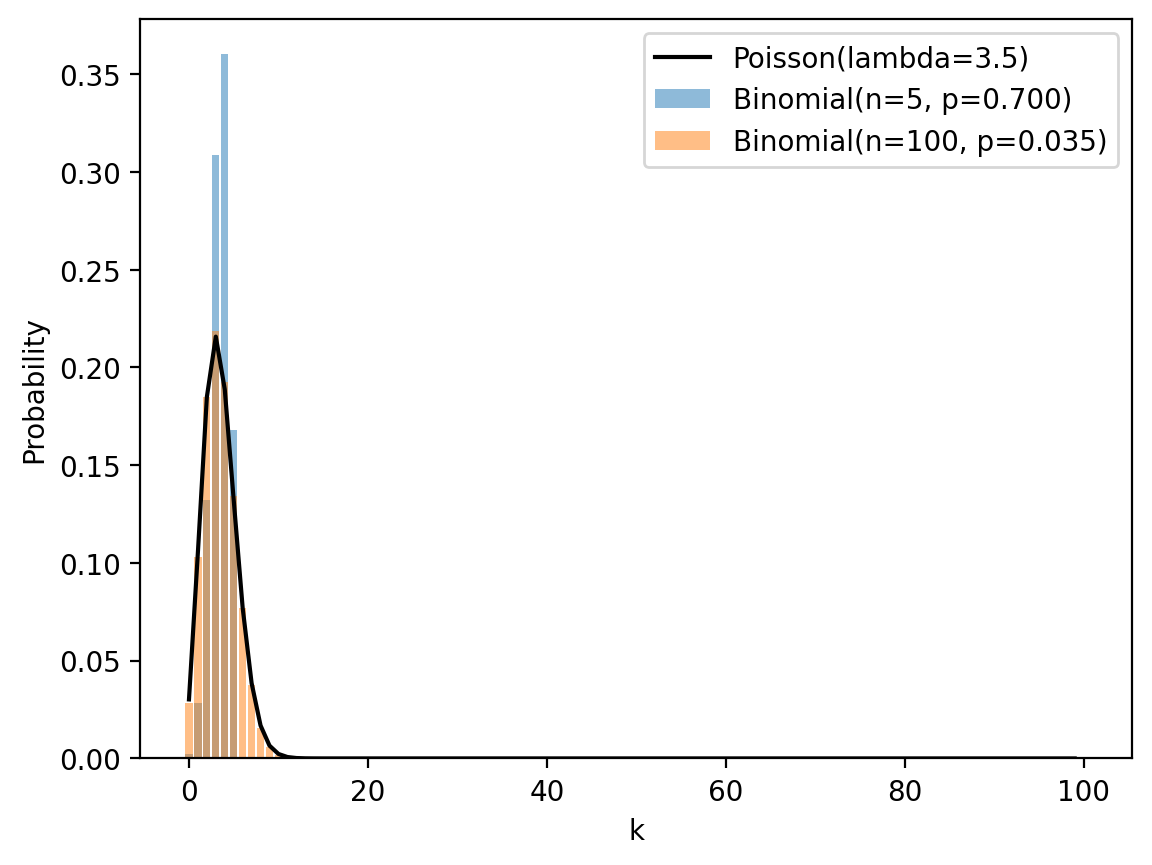
\includegraphics[scale=0.5]{images/poisson_convergence.png}
\raggedright

Notice that as $n$ increases, the peak probability decreases and the tail probabilities increase.
With $n=100$, the shape of the binomial is very close to that of the Poisson.
Also recall that the Poisson is a discrete distribution, but here we have graphed an envelope for clarity.

\begin{theorem}
\textbf{Continuous Mapping Theorem:}
Let $X_n {D \atop \rightarrow} X$ and $g: \mathbb{R} \rightarrow \mathbb{R}$ be continuous.
Then $g(X_n) {D \atop \rightarrow} g(X)$.
\end{theorem}
\begin{proof}
Let $F_n$ be the CDF of $X_n$ and $F$ be the CDF of $X$.
Then the CDF of $g(X_n)$ is $F_n \circ g^{-1}$ and the CDF of $X$ is $F \circ g^{-1}$.
Notice $F_n \circ g^{-1} \rightarrow F \circ g^{-1}$ pointwise.
Thus, $X_n {D \atop \rightarrow} X$.
\end{proof}

\begin{definition}
Let $\{X_n\}_{n=0}^\infty$ be a sequence of random variables and $X$ a random variable.
Say the sequence $X_n$ converges in probability to $X$, $X_n {P \atop \rightarrow}$, whenever for all $\epsilon >0$,
\begin{equation}
\lim_{n\rightarrow \infty} \Pr(|X_n -X|>\epsilon)=0
\end{equation}
\end{definition}

\begin{lemma}
If $X_n {P \atop \rightarrow} X$ and $g: \mathbb{R} \rightarrow \mathbb{R}$ is a continuous and bounded function, $g(X_n) \rightarrow g(X)$.
\end{lemma}


\begin{lemma}
If $X_n {P \atop \rightarrow} X$, then $X_n {D \atop \rightarrow} X$.
\end{lemma}
\begin{proof}
Let $K=\max \{ g(x) | x\in \mathbb{R}\}$.
Also, let $\epsilon>0$ and $A_n$ be the event $\{|g(X_n) - \mathbb{E}(g(X))|>\frac{\epsilon}{2}\}$.
Then
\begin{align*}
\left|\mathbb{E}[g(X_n)] - \mathbb{E}[g(X)]\right|
&= \left|\mathbb{E}\bigl[g(X_n) - \mathbb{E}[g(X)]\bigr]\right| \\
&\le \mathbb{E}\left[\left|g(X_n) - \mathbb{E}[g(X)]\right|\right] \\
&= \int_{\mathbb{R}} \left|g(x) - \mathbb{E}[g(X)]\right| \, dF_n \\
&= \int_{A_n} \left|g(x) - \mathbb{E}[g(X)]\right| \, dF_n
  + \int_{A_n^c} \left|g(x) - \mathbb{E}[g(X)]\right| \, dF_n \\
&\le \int_{A_n} K \, dF_n + \int_{A_n^c} \frac{\epsilon}{2} \, dF_n \\
&= K\,p(A_n) + \frac{\epsilon}{2}\,p(A_n^c).
\end{align*}
Because $X_n {P\atop \rightarrow}X$, $p(A_n)<\frac{\epsilon}{2K}$ for large $n$.
Therefore, $|\mathbb{E}(g(X_n)) - \mathbb{E}(g(X))| \rightarrow 0$.
Finally, we can show this result implies convergence in distribution.
\end{proof}

\end{document}
